\documentclass{beamer}
\usetheme{Szeged}
\usepackage[round,sort]{natbib}
\usepackage{tikz}
\usetikzlibrary{arrows,decorations.pathmorphing,backgrounds,fit,positioning,shapes.symbols,chains}
\usepackage{adjustbox}
\usepackage{verbatim}
\usepackage{graphicx}
\graphicspath{ {mci-term-paper-presentation-images/} }

\title{The effect of inventor mobility on  inventor productivity}
\subtitle{MCI Course Term Paper}
\author{Ashwin Iyenggar}
\institute[Indian Institute of Management Bangalore] 
{
  Corporate Strategy and Policy\\
  Indian Institute of Management Bangalore
}
\date{15 February, 2017}
\subject{Investigating the effects of inventor mobility on  invention complexity\\MCI Course Term Paper}

% \pgfdeclareimage[height=0.5cm]{university-logo}{university-logo-filename}
% \logo{\pgfuseimage{university-logo}}

\AtBeginSubsection[]
{
  \begin{frame}<beamer>{Outline}
    \tableofcontents[currentsection,currentsubsection]
  \end{frame}
}

\begin{document}

\begin{frame}
  \titlepage
\end{frame}

\begin{frame}{Outline}
  \tableofcontents
  % You might wish to add the option [pausesections]
\end{frame}

\section{Introduction}
\begin{frame}{Prior Literature}{Variation in the mobility of inventors across regions}
\begin{itemize}
\item{\cite{Almeida1999} suggested that interfirm mobility of engineers influences the local transfer of knowledge.}
\item{\cite{Ge2016} interpret the higher levels of mobility in silicon valley as the outcome of targeted retention of human capital.}
\item{Unanswered is if the variation in inventor mobility can also explain the variation in innovation productivity in the future.}
\end{itemize}
\end{frame}

\begin{frame}{Research Question}{}
\begin{itemize}
\item{What is the relationship between the movement of some inventors into or out of a region and the average productivity of inventions from those inventors?}
\end{itemize}
\end{frame}

\begin{frame}{Trends}{}
\begin{figure}[h]
\begin{centering}
  \includegraphics[width=0.7\textwidth]{countrymoves}
  \caption{Country moves by year}
   \label{fig:countrymoves}
\end{centering}
\end{figure}
\end{frame}

\begin{frame}{Trends}{}
\begin{figure}[h]
\begin{centering}
  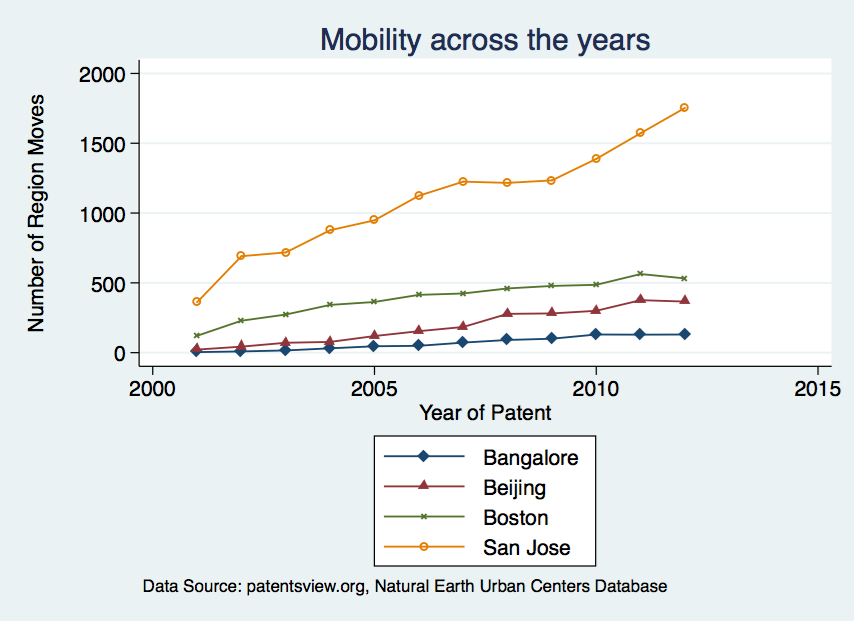
\includegraphics[width=0.7\textwidth]{regionmoves}
  \caption{Region moves by year}
   \label{fig:regionmoves}
\end{centering}
\end{figure}
\end{frame}

\begin{frame}{Statistics}{}
\begin{table}[htbp]\centering \caption{Summary statistics \label{sumstat}}
\begin{tabular}{l c c  c}\hline\hline
\multicolumn{1}{c}{\textbf{Variable}} & \textbf{Mean}
 & \textbf{Std. Dev.} & \textbf{N}\\ \hline
Moved Region (MR) & 0.06 & 0.238  & 4368062\\
Moved Country (MC) & 0.021 & 0.143  & 4368062\\
Productivity & 1.79 & 2.647  & 4368062\\
Prior Patents of Inventor (PPI) & 4.716 & 16.718  & 4368062\\
Prior Patents of Team (PPT) & 24.557 & 112.7  & 3721064\\
\hline
\end{tabular}
\end{table}
\end{frame}

\begin{frame}{Relevance of Answering the Research Question}{}
\begin{itemize}
\item{Received wisdom earlier was that firms would locate themselves in economic agglomerations to benefit from knowledge spillovers \citep{Jaffe1993}.}
\item{\cite{Zhao2006} has argued  that multinational enterprises may benefit from conducting R\&D in countries with weak IPR protection by  making up for the weaker IPR protection through better internal organization.}
\item{The anecdotal increase in the mobility of employees at the weak IPR subsidiaries raises a potential paradox.}
\item{If increased mobility of employees influences transfer of knowledge \citep{Almeida1999}, should we expect higher productivity  from inventors in those teams into which other inventors have moved in?}
\item{The answer to this question is not completely explained by theory}
\end{itemize}
\end{frame}

\begin{frame}{Managerial and Policy Implications}{}
\begin{itemize}
\item{The innovation policy of emerging countries is influenced with the expectation that the presence of multinational R\&D will create value adding spillover effects.}
\item{Productivity of innovation provides a richer proxy for value adding innovation, and effects of inventor mobility may inform innovation policy}
\item{Current work may inform managerial decisions about how to organize R\&D teams around the world}
\end{itemize}
\end{frame}

\section{Theory}
\begin{frame}{Hypotheses}{}
\begin{itemize}
\item{H1: An increase in the average mobility of inventors in a region increases the average productivity of  the inventor}
\item{H2: The effect in H1 is moderated positively by the strength of the prior pool of inventions by the inventor}
\item{H3: The effect in H1 is moderated negatively by the strength of the prior pool of inventions by the inventing team}
\end{itemize}
\end{frame}


\section{Data and Method}
\begin{frame}{Methodology}{}
\begin{itemize}
\item{Data Source: Patents from USPTO, source: patentsview.org}
\item{Unit of Analysis: Inventor-Year}
\item{Dependent Variable: Productivity of inventor in a year}
\item{Primary Explanatory Variable: Mobility of innovators (Between-Region Mobility, Between-Country Mobility)}
\item{Moderating Variables: Prior patents of inventor (PPI), Prior patents of team (PPT) }
\item{Control Variables: Technology subcategories,  Year effects}
\end{itemize}
\end{frame}

\begin{frame}{Results}{}

\end{frame}

\begin{frame}{Potential Issues}{}
\begin{itemize}
\item{Direction of Causality}
\item{Underestimation bias of mobility - effects}
\item{Mechanism by which mobility affects productivity - other explanations}
\item{Alternative measures of productivity }
\end{itemize}
\end{frame}



\bibliography{/Users/aiyenggar/OneDrive/code/bibliography/ae,/Users/aiyenggar/OneDrive/code/bibliography/fj,/Users/aiyenggar/OneDrive/code/bibliography/ko,/Users/aiyenggar/OneDrive/code/bibliography/pt,/Users/aiyenggar/OneDrive/code/bibliography/uz}
\bibliographystyle{apalike}

\end{document}

\begin{comment}
\begin{figure}[h]
\begin{centering}
  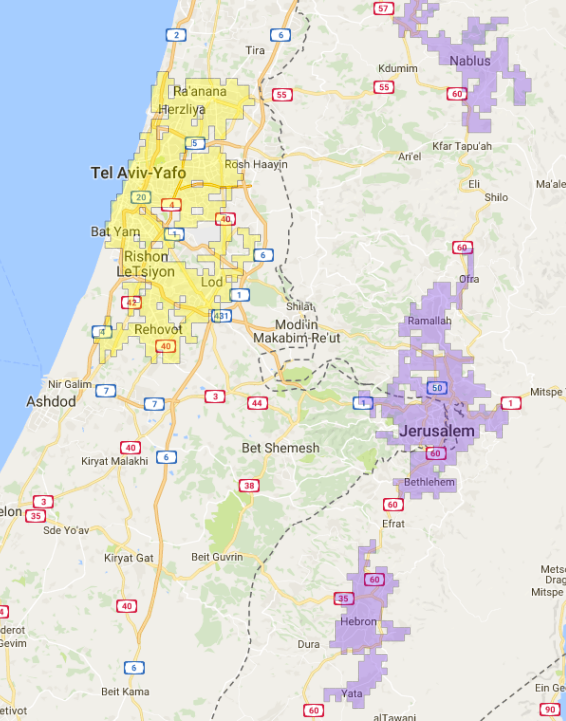
\includegraphics[width=\textwidth]{TelAviv}
  \caption{Geographic Definition of Tel Aviv-Yafo}
   \label{fig:TelAviv}
\end{centering}
\end{figure}
\end{comment}

